\documentclass[journal]{IEEEtran}

\usepackage[T1]{fontenc}
\usepackage[utf8]{inputenc}
\usepackage{amsmath,amssymb,amsfonts}
\usepackage{graphicx}
\usepackage{booktabs}
\usepackage{array}
\usepackage{url}
\usepackage{xcolor}
\usepackage[hidelinks]{hyperref}
\usepackage{orcidlink}
\usepackage{balance}

\graphicspath{{../figures/}}

\renewcommand{\topfraction}{0.92}
\renewcommand{\bottomfraction}{0.75}
\renewcommand{\textfraction}{0.08}
\renewcommand{\floatpagefraction}{0.80}

% IEEEtran hard-codes an em-dash after the abstract and index-terms names; the CAOS
% content standard (ADR-0067) excludes em-dashes, so the separator is a full stop.
\makeatletter
\def\abstract{\normalfont
    \if@twocolumn
      \@IEEEabskeysecsize\bfseries\textit{\abstractname}.\ \relax
    \else
      \bgroup\par\addvspace{0.5\baselineskip}\centering\vspace{-1.78ex}\@IEEEabskeysecsize\textbf{\abstractname}\par\addvspace{0.5\baselineskip}\egroup\quotation\@IEEEabskeysecsize
    \fi\@IEEEgobbleleadPARNLSP}
\def\IEEEkeywords{\normalfont
    \if@twocolumn
      \@IEEEabskeysecsize\bfseries\textit{\IEEEkeywordsname}.\ \relax
    \else
      \bgroup\par\addvspace{0.5\baselineskip}\centering\@IEEEabskeysecsize\textbf{\IEEEkeywordsname}\par\addvspace{0.5\baselineskip}\egroup\quotation\@IEEEabskeysecsize
    \fi\@IEEEgobbleleadPARNLSP}
\makeatother

% Page-1 header block (conventions/manuscript-header-standard.md). The four document
% macros are set by the publishing tool when the version DOI is reserved.
\newcommand{\doctype}{Technical report}
\newcommand{\docversion}{v1.1}
\newcommand{\docdate}{18 September 2026}
\newcommand{\versiondoi}{10.5281/zenodo.22822962}
\newcommand{\conceptdoi}{10.5281/zenodo.21512647}
\newcommand{\docrepo}{github.com/fsantibanezleal/CAOS\_QLAB}
\newcommand{\headerblock}{%
\begin{center}
\fbox{\parbox{0.94\textwidth}{\small\raggedright
\textbf{\doctype} \quad$\cdot$\quad \docversion, \docdate \quad$\cdot$\quad Licence CC BY 4.0\\[2pt]
CAOS open-research programme \quad$\cdot$\quad QLab, quantum-versus-classical benchmarking laboratory\\[2pt]
Version DOI \href{https://doi.org/\versiondoi}{\texttt{\versiondoi}} \quad$\cdot$\quad
concept DOI (always latest) \href{https://doi.org/\conceptdoi}{\texttt{\conceptdoi}}\\[2pt]
Not peer reviewed. Source code, data and computational records: \href{https://\docrepo}{\texttt{\docrepo}}
}}
\end{center}}

\begin{document}

\title{Classical Still Wins the Wall-Clock:\\ A Quantum-vs-Classical Benchmark of Twenty\\ Canonical Problems on Five Real Frameworks}

\author{Felipe~Santiba\~nez-Leal~\orcidlink{0000-0002-0150-3246}%
\thanks{F. Santiba\~nez-Leal is with the CAOS open-research programme, Santiago, Chile
(e-mail: fsantibanez@gmail.com; ORCID 0000-0002-0150-3246).}%
\thanks{Interactive laboratory and reproducible traces (MIT) at
\url{https://github.com/fsantibanezleal/CAOS_QLAB}; the laboratory is available at
\url{https://qlab.fasl-work.com}.}}

\markboth{\doctype\ \docversion, 2026 \textperiodcentered\ CAOS open-research programme}%
{Santiba\~nez-Leal: A quantum-vs-classical benchmark on five real frameworks}

\IEEEaftertitletext{\vspace{-0.6\baselineskip}\headerblock\vspace{0.2\baselineskip}}

\maketitle

\begin{abstract}
Demonstrations of quantum algorithms often stop at a toy circuit and report no classical baseline. This report
formulates twenty canonical quantum problems, attacks each with the real, dedicated frameworks (Qiskit with Aer, PennyLane, Cirq, Stim, and
NumPy/scikit-learn for the classical baselines), and puts every quantum method next to its classical baseline
with both costs on the table. The result, from $119$ archived, reproducible traces, is unambiguous:
at lab scale the classical baseline is faster in wall-clock time on \emph{all twenty} problems, usually by two to
four orders of magnitude, and this holds even for the flagship ``advantage'' algorithms, Grover's search and
Shor's factoring, because their asymptotic advantages do not materialise at the small instance sizes a laptop
simulator reaches. Yet the quantum phenomena are real, and the benchmark reproduces them: the CHSH value reaches the
Tsirelson bound $2\sqrt{2}$ and violates the classical local-hidden-variable bound of $2$ (but only with
entanglement; a separable state gives $1.41$), Grover uses provably fewer oracle queries ($2$ versus $7$ on one
instance), and Shor's order-finding factors $15$ correctly. In summary, on these twenty problems the quantum
methods win at \emph{physics} (nonlocality, query complexity) and not at \emph{wall-clock computation} at the
instance sizes a simulator reaches, and the benchmark shows why, with measured numbers on real frameworks,
reproducibly.
\end{abstract}

\begin{IEEEkeywords}
Quantum computing, quantum advantage, benchmarking, Grover, Shor, CHSH, Bell inequality, QAOA, VQE, NISQ,
reproducibility, classical baselines.
\end{IEEEkeywords}

\section{Introduction}

\IEEEPARstart{D}{emonstrations} of quantum algorithms often omit the comparison that decides whether a
method is useful: a tutorial runs a Bell pair or a two-qubit Grover and stops, and a benchmark reports a quantum
method's accuracy without running the classical baseline next to it. The research literature states that
near-term quantum hardware is noisy and limited~\cite{preskill,bharti}, and the headline results (quantum
supremacy on a sampling task engineered to be hard for classical machines~\cite{arute}) concern a task chosen
for classical hardness rather than a useful problem. This report makes the comparison concrete and
reproducible: it takes the problems quantum computing is usually taught on, runs them on the real frameworks,
puts the classical baseline beside each one, and reports the measured numbers.

The laboratory behind this report, QLab, is a small Problem\,$\times$\,Solver engine. A \emph{problem} is a
formulation (search, factoring, ground-state energy, a Bell test) with its instances and observable; a
\emph{solver} is a thin adapter over a real framework: Qiskit with the Aer simulator, PennyLane, Cirq, and Stim
for the quantum methods, and NumPy with scikit-learn for the classical baselines. Every run records its cost
(qubits, gates, shots, wall-time) and its result, and the traces are archived in the repository so that every
number can be checked. Over twenty problems and $119$ archived traces the engine answers one question for each:
run on the best real framework available, does the quantum method beat the classical baseline, and at what cost?
The answer is the subject of this report.

% Defined here so that the two-column float is placed at the top of page 2, beside Section III.
\begin{figure*}[!t]
\centering
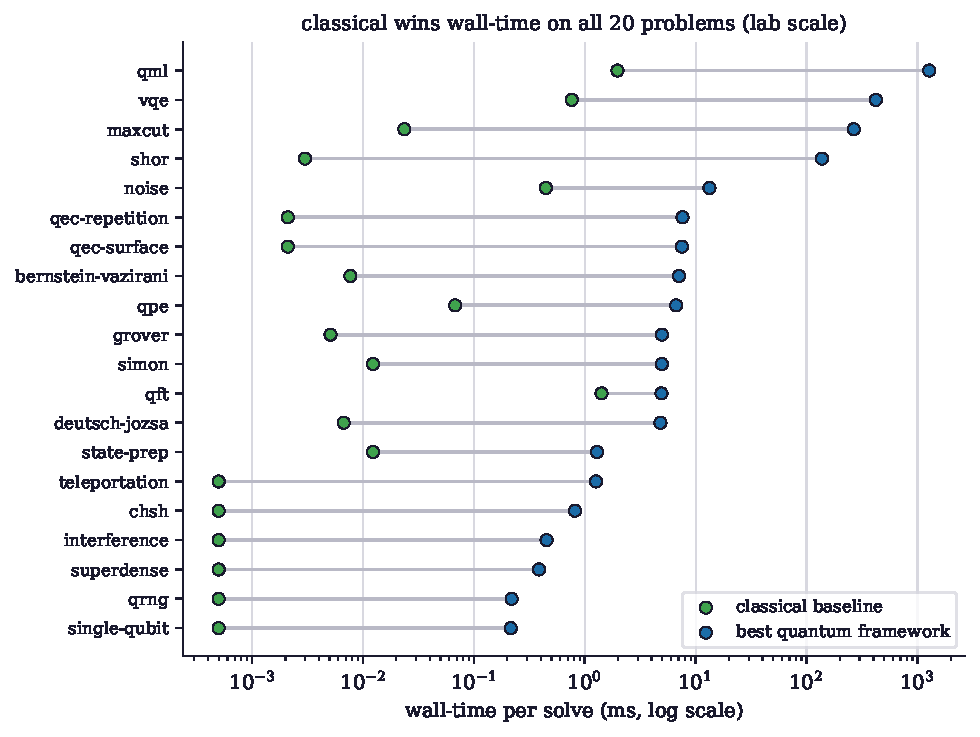
\includegraphics[width=0.7\textwidth]{fig-walltime.pdf}
\caption{Wall-time per solve, classical baseline versus the best quantum framework, on each of the twenty
problems (log scale; problems sorted by quantum wall-time). The classical baseline (green) is faster on
\emph{every} problem, usually by two to four orders of magnitude, from microseconds against $0.4$ to $7$~ms on the
oracle and entanglement cases to at most $2$~ms against $266$ to $1274$~ms on the variational
cases (QAOA, VQE, quantum machine learning). This includes the flagship algorithms: Shor factoring $15$ and
Grover search are both far cheaper to run classically at this scale.}
\label{fig:walltime}
\end{figure*}

\section{The Benchmark: Twenty Problems, Five Frameworks}\label{sec:bench}

The twenty problems span the standard curriculum: single-qubit and interference fundamentals; entanglement
(Bell/CHSH, teleportation, superdense coding, state preparation); the oracle algorithms (Deutsch--Jozsa,
Bernstein--Vazirani, Simon); the flagship algorithms (Grover's search~\cite{grover}, Shor's
factoring~\cite{shor}, the quantum Fourier transform, quantum phase estimation); the variational methods (QAOA
for MaxCut~\cite{farhi}, VQE~\cite{peruzzo}, a small quantum-machine-learning classifier); and noise and quantum
error correction (a repetition code and a surface-code round, simulated with the dedicated stabilizer simulator
Stim~\cite{stim}). Each problem is solved by every applicable framework and by a classical baseline, under a
fixed seed and shot budget, and the resulting trace records the outcome and the full cost. The costs are what
make the comparison fair: a quantum method that gets the right answer is not ``winning'' if it needs a hundred
times the wall-time of a classical routine that also gets the right answer, and the trace shows both side by
side. All traces run on classical simulators of the quantum circuits, the regime a public laboratory can reach;
this is the correct regime for the lab-scale question the report asks.

\section{The Wall-Clock Result: Classical Wins All Twenty}\label{sec:walltime}

The headline result is Fig.~\ref{fig:walltime} and Table~\ref{tab:cases}: on all twenty problems, the classical
baseline is faster in wall-clock time than the best real quantum framework, at the instance sizes a simulator
reaches. The margins are large. On the entanglement and oracle problems the classical routine finishes in at most
$12.3$~microseconds, while the quantum framework takes $0.39$ to $1.3$~ms on the entanglement problems and $4.8$ to
$7.1$~ms on the oracle problems, a gap of about $100$ to more than $1000$ times dominated by circuit construction
and simulation overhead. On the variational problems the gap is starkest: classical MaxCut
by brute force takes $0.02$~ms against QAOA's $266$~ms, and the classical VQE and quantum-machine-learning
baselines finish in $0.76$ and $1.97$~ms against $420$ and $1274$~ms for their quantum counterparts. Even the two
algorithms whose entire fame is a speedup lose here: Shor's order-finding factors $15$ in $137$~ms while trial
division does it in $3$~microseconds, and Grover's search costs more wall-time than a classical scan of eight
items. This is not a bug and not a slow implementation; it is the expected consequence of asking
small-instance questions, where a quantum algorithm's asymptotic advantage is nowhere near paying for the
constant-factor overhead of building and simulating a circuit.

\begin{table}[!t]
\centering
\caption{The twenty problems, representative instance: classical vs best-quantum wall-time (ms) and the quantum
framework(s). Classical is faster on all twenty. Full costs (qubits, gates, shots) are in the archived traces.}
\label{tab:cases}
\scriptsize
\begin{tabular}{@{}l l r r@{}}
\toprule
Problem & category & classical (ms) & quantum (ms) \\
\midrule
single-qubit        & fundamentals   & $<0.001$ & $0.22$ \\
qrng                & fundamentals   & $<0.001$ & $0.22$ \\
interference        & fundamentals   & $<0.001$ & $0.45$ \\
superdense          & entanglement   & $<0.001$ & $0.39$ \\
teleportation       & entanglement   & $<0.001$ & $1.26$ \\
chsh                & entanglement   & $<0.001$ & $0.82$ \\
state-prep          & entanglement   & $0.012$ & $1.29$ \\
deutsch-jozsa       & oracle         & $0.007$ & $4.81$ \\
bernstein-vazirani  & oracle         & $0.008$ & $7.08$ \\
simon               & oracle         & $0.012$ & $4.94$ \\
grover              & flagship       & $0.005$ & $4.96$ \\
qft                 & flagship       & $1.42$ & $4.91$ \\
qpe                 & flagship       & $0.068$ & $6.66$ \\
shor                & flagship       & $0.003$ & $137.4$ \\
maxcut (QAOA)       & variational    & $0.024$ & $266.0$ \\
vqe                 & variational    & $0.76$ & $420.6$ \\
qml                 & variational    & $1.97$ & $1273.6$ \\
qec-repetition      & noise/QEC      & $0.002$ & $7.6$ \\
qec-surface         & noise/QEC      & $0.002$ & $7.5$ \\
noise               & noise/QEC      & $0.45$ & $13.3$ \\
\bottomrule
\end{tabular}
\end{table}

\section{Where Quantum Wins: Physics, Not Wall-Time}\label{sec:phenomena}

\begin{figure*}[!t]
\centering
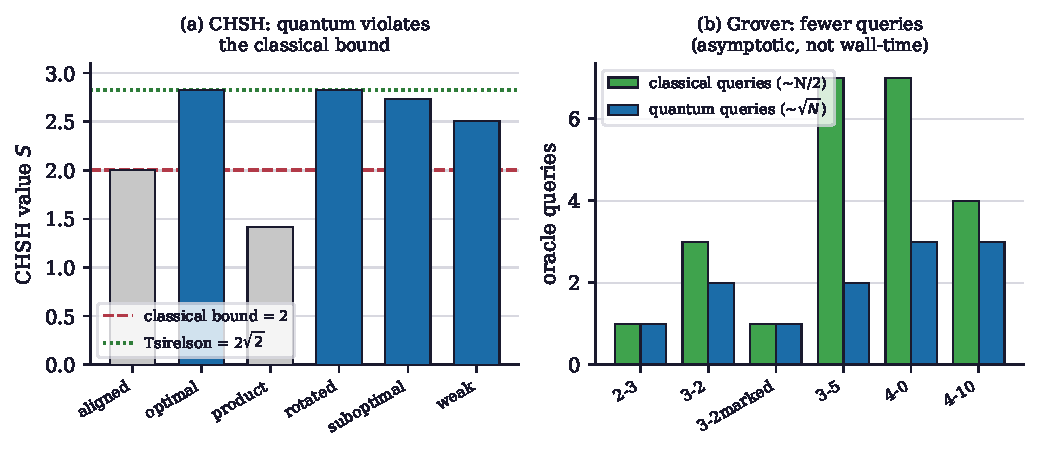
\includegraphics[width=0.9\textwidth]{fig-phenomena.pdf}
\caption{The quantum phenomena the benchmark demonstrates: real, but not yet a wall-time advantage.
\textbf{(a)} The CHSH value $S$ across measurement settings: the optimal and rotated settings reach the
Tsirelson bound $2\sqrt{2}\approx2.83$ and \emph{violate} the classical local-hidden-variable bound of $2$, but
only with entanglement; a product (separable) state gives $S=1.41$ and the aligned setting sits exactly at $2$.
\textbf{(b)} Grover's oracle-query count versus a classical scan: quantum uses provably fewer queries (two versus
seven on the three-qubit, one-marked instance), the quadratic $\sqrt{N}$ advantage, which is real in query
complexity even though it does not beat the classical wall-time at this $N$.}
\label{fig:phenomena}
\end{figure*}

That classical wins the wall-clock does not mean quantum does nothing; it means the win is in physics, not
practical computation, and the benchmark shows exactly where (Fig.~\ref{fig:phenomena}). The clearest case is the
CHSH/Bell test~\cite{clauser}. With entangled qubits and the optimal measurement settings the correlator sum
reaches $S=2.83$, the Tsirelson bound~\cite{tsirelson}, and \emph{violates} the classical bound of $2$ that any
local-hidden-variable theory must obey, exactly the violation whose experimental realisation~\cite{aspect} earned
the 2022 Nobel Prize. This is a quantum-beats-classical result, but it is a statement about the structure
of nature (local realism is false), not a faster computation, and it requires entanglement: the benchmark's
product-state variant gives $S=1.41$ and does not violate anything. The second case is query complexity: Grover's
algorithm~\cite{grover} finds a marked item in about $\sqrt{N}$ oracle queries against a classical scan's $N/2$,
and the benchmark measures the advantage directly (two quantum queries against seven classical on one instance).
This too is real, a proven separation in the number of oracle calls, and it too fails to beat wall-time at
reachable $N$ because each quantum query costs far more to simulate than a classical array lookup. Shor's
algorithm~\cite{shor} completes the picture: it factors $15$ correctly through order-finding, a correct execution
of a quantum algorithm, while remaining, at the scale that matters, no threat: factoring RSA-2048 would
need on the order of a million noisy physical qubits with full fault tolerance~\cite{gidney}, which is why
Shor's algorithm is not a near-term cryptographic danger.

\section{Discussion}\label{sec:discuss}

The benchmark separates two questions. \emph{Does quantum mechanics do things classical physics cannot?} Yes,
and the CHSH violation is the clean demonstration. \emph{Does a quantum computer beat a classical one in
wall-clock time on these problems, at the instance sizes a simulator reaches?} No, on all twenty problems, and
the wall-times say so, usually by two to four orders of magnitude. The two answers are not in tension, and
putting them side by side shows a learner both the physics and the cost of computing with it at this scale. The
report also makes a methodological point: a quantum-vs-classical comparison is only meaningful with the
classical baseline actually run and its cost reported, and an asymptotic advantage cannot be observed on an
instance far too small for it to appear. The benchmark builds this requirement into the architecture: every
quantum solver has a classical sibling, and both costs are always on screen.

\section{Scope and Limitations}\label{sec:limits}

Every trace runs on a \emph{classical simulator} of the quantum circuit, not on quantum
hardware; this is the regime a public laboratory can reach and is the correct regime for the lab-scale question,
but it means the wall-times measure simulation cost, not a physical quantum processor, and a fault-tolerant
machine at large scale would change the asymptotic story for Shor and for quantum chemistry (not demonstrated
here, and not claimed). The instances are small (a handful of qubits), by necessity, so the benchmark measures
the small-$N$ regime where asymptotic advantages are absent by construction; it does not and cannot refute the
existence of a large-$N$ advantage, only show that it is not present at lab scale. The noise and
error-correction cases are idealised-to-realistic simulator models, not device calibration data. And the
frameworks are pinned versions; a newer release could shift the constants. The laboratory states the same scope
on every panel; the report measures the small-scale regime and makes no claim about the ultimate limits of
quantum computing.

\section{Conclusion}

Run with the classical baseline beside every quantum method and both costs on the table, twenty
canonical quantum problems on five real frameworks give one answer: at lab scale the classical baseline wins the
wall-clock on all twenty, including the flagship speedup algorithms, because their advantages are asymptotic and
the instances are small. And yet quantum wins at physics: the CHSH bound is violated, Grover's query
advantage is real, Shor factors correctly. On these problems, quantum methods beat classical ones at
nonlocality and query complexity but not in wall-clock time at lab scale, and the benchmark shows this
reproducibly, with measured numbers on real frameworks.

\appendices
\section{Reproduction}\label{app:repro}

{\raggedright
The benchmark is the $119$ traces archived under \path{data/artifacts/}, one folder per problem, each trace
recording the problem, the solvers, the per-solver costs, and the quantum-vs-classical outcome. The
aggregation script (\path{manuscripts/quantum-vs-classical/figures/aggregate.py}) walks them into the summary
artifact the figures read, extracting the per-problem wall-times, the CHSH value across settings, and the Grover
query counts. Re-running the traces (each is seeded) reproduces the numbers; the figures and
Table~\ref{tab:cases} regenerate from the archived summary
(\path{manuscripts/quantum-vs-classical/data/bench_summary.json}).\par}

\balance

\begin{thebibliography}{00}

\bibitem{preskill} J.~Preskill, ``Quantum computing in the NISQ era and beyond,'' \emph{Quantum}, vol.~2,
art.~79, 2018. doi:10.22331/q-2018-08-06-79.

\bibitem{bharti} K.~Bharti \emph{et al.}, ``Noisy intermediate-scale quantum algorithms,'' \emph{Reviews of
Modern Physics}, vol.~94, art.~015004, 2022. doi:10.1103/RevModPhys.94.015004.

\bibitem{arute} F.~Arute \emph{et al.}, ``Quantum supremacy using a programmable superconducting processor,''
\emph{Nature}, vol.~574, pp.~505--510, 2019. doi:10.1038/s41586-019-1666-5.

\bibitem{grover} L.~K. Grover, ``A fast quantum mechanical algorithm for database search,'' in \emph{Proc. 28th
Annual ACM Symp. Theory of Computing (STOC)}, 1996, pp.~212--219. doi:10.1145/237814.237866.

\bibitem{shor} P.~W. Shor, ``Polynomial-time algorithms for prime factorization and discrete logarithms on a
quantum computer,'' \emph{SIAM Journal on Computing}, vol.~26, no.~5, pp.~1484--1509, 1997.
doi:10.1137/S0097539795293172.

\bibitem{gidney} C.~Gidney, ``How to factor 2048 bit RSA integers with less than a million noisy qubits,'' 2025.
arXiv:2505.15917.

\bibitem{farhi} E.~Farhi, J.~Goldstone, and S.~Gutmann, ``A quantum approximate optimization algorithm,'' 2014.
arXiv:1411.4028.

\bibitem{peruzzo} A.~Peruzzo \emph{et al.}, ``A variational eigenvalue solver on a photonic quantum processor,''
\emph{Nature Communications}, vol.~5, art.~4213, 2014. doi:10.1038/ncomms5213.

\bibitem{clauser} J.~F. Clauser, M.~A. Horne, A.~Shimony, and R.~A. Holt, ``Proposed experiment to test local
hidden-variable theories,'' \emph{Physical Review Letters}, vol.~23, no.~15, pp.~880--884, 1969.
doi:10.1103/PhysRevLett.23.880.

\bibitem{tsirelson} B.~S. Cirel'son, ``Quantum generalizations of Bell's inequality,'' \emph{Letters in
Mathematical Physics}, vol.~4, no.~2, pp.~93--100, 1980. doi:10.1007/BF00417500.

\bibitem{aspect} A.~Aspect, P.~Grangier, and G.~Roger, ``Experimental realization of Einstein--Podolsky--Rosen--
Bohm gedankenexperiment: A new violation of Bell's inequalities,'' \emph{Physical Review Letters}, vol.~49,
no.~2, pp.~91--94, 1982. doi:10.1103/PhysRevLett.49.91.

\bibitem{stim} C.~Gidney, ``Stim: A fast stabilizer circuit simulator,'' \emph{Quantum}, vol.~5, art.~497, 2021.
doi:10.22331/q-2021-07-06-497.

\end{thebibliography}

\end{document}
